% This must be in the first 5 lines to tell arXiv to use pdfLaTeX, which is strongly recommended.
\pdfoutput=1
% In particular, the hyperref package requires pdfLaTeX in order to break URLs across lines.

\documentclass[11pt]{article}
\usepackage{graphicx}
\usepackage{wrapfig}
\usepackage{amsmath}

% Remove the "review" option to generate the final version.
\usepackage[]{ACL2023}

% Standard package includes
\usepackage{times}
\usepackage{latexsym}

% For proper rendering and hyphenation of words containing Latin characters (including in bib files)
\usepackage[T1]{fontenc}
% For Vietnamese characters
% \usepackage[T5]{fontenc}
% See https://www.latex-project.org/help/documentation/encguide.pdf for other character sets

% This assumes your files are encoded as UTF8
\usepackage[utf8]{inputenc}

% This is not strictly necessary, and may be commented out.
% However, it will improve the layout of the manuscript,
% and will typically save some space.
\usepackage{microtype}

% This is also not strictly necessary, and may be commented out.
% However, it will improve the aesthetics of text in
% the typewriter font.
\usepackage{inconsolata}

\title{Assessing the Impact Score of Scientific Publications through the Analysis of Abstracts and their Metadata}

\author{Artem Lebedev\\
  UC Berkeley / Berkeley, CA \\
  \texttt{artem.lebedev@berkeley.edu} \\\And
 Farouk Ghandour \\
  UC Berkeley / Berkeley, CA \\
  \texttt{fghandour18@berkeley.edu} \\}

\begin{document}
\maketitle

\begin{abstract}
An impact score of the academic paper is a metric critically important for a scientist's career and attraction of funding for future research. The ability to predict the potential score of a paper could help scientists adjust their presentation strategy to achieve maximum impact. Natural language processing (NLP) is a logical tool to examine what leads to a scientific article's strong impact score because it allows one to analyze an article’s content numerically. In this paper we investigate if the content of the abstract matters for the selection of the journal, or meta-factors, such as author address and number of co-authors are sufficient to select the bset possible journal for submission.\footnote{The code and data available on \href{https://github.com/ArtemChemist/w266_project}{GitHub} and \href{https://drive.google.com/drive/folders/1OkSzswtFvqA6_FD35vvSCU31kSd1ECA2?usp=drive_link}{GDrive}.}
\end{abstract}

\section{Introduction}
A measurement of the academic paper's impact is critically important for a scientist's career and attraction of funding for future research. The ability to predict the paper's significance could help researchers adjust their presentation strategy to achieve maximum visibility. Our team aims to elucidate the factors that drive acceptance in high-impact journals.

Our hypothesis is that variation in the impact of an academic paper can be mostly explained by the metadata of the paper: country of origin, number of authors, length of the paper etc. The metrics of impact that is the most amenable for the quantitative analysis is Journal Impact Factor (JIF), wich is, roughly, the average number of times papers in the journals are cited in the works of others.   

We selected Pearson's correlation coefficient between the predicted impact and observed impact as the metric to evaluate and compare models. We will assume that we failed to reject null hypothesis if observed-predicted correlation of the model including text data and metadata is not significantly larger than correlation achieved with the same model lacking text data (Eq.~\ref{eq:hypothesis}).
\begin{equation}\label{eq:hypothesis}
	\begin{cases}
		H_{0}: (r_{w\ text} - r_{only\ metadata}) \leq 0 \\
		H_{A}: (r_{w\ text} - r_{only\ metadata}) > 0\\
	\end{cases}       
\end{equation}
In the social science context correlation coefficient above 0.5 is generally considered moderately positive\citep{KahnemanDaniel2021N:af}. Following this convention, we will consider our findings to be practically significant only if at least one coefficient exceeds 0.5. If both coefficients are below 0.5, it is likely that our research question can not be answered with this data set and our approach. 

\section{Background}
% Not done. Supppoesed to describe motivation for the work.
A few attempts have been made to address this issue, demonstrating modest but encouraging success. \citep{Macri2023-tr, Alohali2022-no, 10.1162/qss_a_00258, doi:10.1152/japplphysiol.00489.2020} The most sophisticated model utilized BERT context-aware encoding of the abstract to produce embedding that were then classified using  SVM, logistic regression or XGBoost to predict the impact factor quintile. This approach demonstrated prediction accuracy of approx. 75%.

\section{Data}
We extracted data from the Web of Science, a platform that provides access to citation metrics for the majority of life science publications. The platform provides csv files with the article abstract along with the ISSN identifier of the journal and other metadata. To reduce variability unrelated to the research question we focus on a narrow field of radioligand therapy and select only original peer-reviewed articles published in English between 2000 and 2022. JIFs are available from Claritive Analytics “Journal Impact Factor Report” and contain the journal ISSN as well as the impact factor, by year. Merging these two datasets on ISSN we achieve our raw dataset, containing approximately 4500 records.

Since our aim is to support researcher decision on publication strategy, we focus on the features available to authors at the time of submission: 'Year Published', 'Authors', 'Document Title', 'Author Keywords', 'Abstract', 'Author Address', 'Funding Agency and Grant Number', 'Cited Reference Count', 'Page Count'. Using author identities as features would result in very sparse set of categorical variables, therefore we reduced the author information to just the number of authors and the author address to just the country. We also reduced the funding information to a binary variable funded/not-funded. 'Abstract' is the most important and relevant feature of the paper. Together with the title and author's keywords it represents condensed meaning of the paper.  
 
EDA revealed that numerical variables are mostly uncorrelated with each other and label is roughly normally distributed around mean of 4.09 with standard deviation of 2.21. Less that 0.1\% of the papers had JIF > 20, but some reached JIF as high as 86. To avoid undue influence of these high performers we filtered out all papers with JIF above 20. Unsurprisingly, USA and the UK dominate the countries of author's origin, but in total more than 80 countries were represented. Majority of abstracts are less that 400 words long with noticeable peak around 250, a popular cut-off required by publishers. For the purpose of tokenization we set 400 tokens a the max length. Some abstracts contained publisher's copyright statements that we removed to avoid a leak from label to the features. Full EDA is available in EDA.ipynb notebook in the project github repository. 

\section{Methods}
We use regression models based on neural networks to predict the impact of the publications. To evaluate the importance of text data, we compare predictive power of the model that includes text data vs the model that is based solely on metadata. Pearson's correlation coefficient between observed and predicted impact values is a metric we use to test our hypothesis. 

Features selected after EDA fall into three general categories: numerical features, categorical features and text. While numerical features can be included into the model as-is, categorical variables and text need to be transformed before they become inputs into neural network. One-hot-encoded representation is a common way to transform categorical variables, but it lacks the ability to capture patterns present in the data. For instance, papers originating from Canada are likely similar to ones written in the USA, but very different from papers submitted from China. To preserve these patterns, we have chosen to use learned embedding representation of the categorical variables \citep{DBLP:journals/corr/GuoB16}.

Transformation of text into contextually-aware embedding is commonly achieved using BERT \citep{DBLP:journals/corr/abs-1810-04805}. sciBERT, a similar model trained on the large corpus of medical and scientific literature, was recently presented \citep{DBLP:journals/corr/abs-1903-10676} and we plan to compare these two models. Both variants of BERT yield several vectors that can represent the text: pooled vector, cls vector or a set of vectors for each input token. For the baseline model we concatenated all three vectors and used them as input into a linear regression. We also investigated using all word embeddings in the model, rather than relying on the summarization tokens produced by BERT model.

\section{Results and discussion}
\subsection{Testing of the main hypothesis}
\textbf{Preliminary experiments} Before testing our hypothesis we tested a few model architecture choices. First we investigated how the number of dense layers affects performance. We used \textit{cls} token generated by standard uncased BERT and added no dense layers, one or two dense layers on top of the 768-dimensional vector. All dense layers had 768 neurons. Correlation between predicted and observed JIFs improved upon addition of the first layer (r = 0.54 vs 0.57 p = 8e-05 after Fisher's transformation, one-tailed, assuming dependent samples), but did not improve with addition of the second dense layer (r = 0.56). Replacing standard BERT with sciBERT, a model trained on scientific text, we further improved the result (r = 0.57 vs 0.64 p = 2e-08). In a separate experiment we demonstrated that use of \textit{cls} token for this regression problem is preferred over the pooled token.

\textbf{Main hypothesis testing} For the baseline model we built three regression models. The one based on metadata only included numerical features concatenated with learned embeddings for each of the categorical features. The resulting vector was fed directly into the dense output layer with one element and linear activation.  Supporting intuition behind our null-hypothesis, r value for this model was 0.55, far better than a random guess. This indicates that metadata alone, with no features related to the essence of the paper, can predict the impact of the paper. The second model included only sciBERT \textit{cls} token and no meta data. This model exhibited r-value of 0.63, a statistically significant (p=0.0008, independent samples) improvement. The final model included both metadata and sciBERT \textit{cls} token concatenated into one vector before the final dense and regression layer. This model demonstrated r = 0.67, an improvement over both baseline models. It exceeded performance of the pure metadata model with p-value 2E-07. Based on that we can reject the null hypothesis and conclude that addition of a feature related to the paper actual meaning increased model's predictive power by approx. 20\%.
Figure~\ref{fig:meta_no_meta} shows the distribution of the observed and predicted JIFs for the first and the third model. Interestingly, both models are reluctant to predict low JIFs. Additionally, learning curves showed clear signs of over-fitting with validation loss far exceeding training loss. 
\begin{figure}
	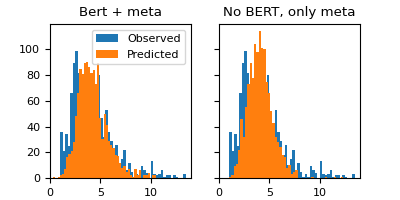
\includegraphics[width= \columnwidth]{./Images/meta no meta.png}
	\caption{Observed-Predicted for models w metadata.}
	\label{fig:meta_no_meta}
\end{figure}

\textbf{Rank prediction} As a first attempt to improve our model, we added drop-out layers after learned embeddings for categorical variables and also tried predicting relative ranking of the paper rather than JIF directly. To that end we calculated the proportion of papers that have the same or lower JIF for each paper (rank). We used max and min JIF obtained from training data and assumed it is representative of the whole population. Scaling label to (0,1) allowed us to use sigmoid activation in the regression layer, which we hoped would make model more sensitive to the changes in the middle of the distribution. However, this approach resulted in lower model performance (r=0.61). Using linear activation instead of sigmoid resulted in even worse performance. The only improvement that we obtained in these experiments is reduced over-fitting: validation loss exceeded training loss later in the training, pointing to the usefulness of the dropout layers.

\subsection{Performance improvement}
In attempt to increase predictive power of the model we hypothesized that incorporating the full set of BERT tokens would allow for better modeling of the abstract meaning. Two general approaches were investigated: using LSTM as an encoder to summarize the abstract and using a CNN set of layers to do the same.

\textbf{LSTM for abstract representation} The intuition behind using LSTM comes from observation that reviewer reads the words one after another to produce their opinion on weather to recommend the paper for publication or not. Just like an LSTM model, the reviewer reads words in sequence and updates the memory of what they read with every word. In the end the final representation of what they read becomes the basis for accept/reject decision. Mimicking this process we built an two-layer LSTM model with 768 nodes (to match BERT embedding) and trained it on the full output of sciBERT (400 tokens). Surprisingly, the correlation between predicted and observed JIFs was only r = 0.57 (\href{https://github.com/ArtemChemist/w266_project/blob/main/Notebooks/sciBERT%20w%20meta%20to%20LSTM.ipynb}{notebook}), substantially lower than the model that used \textit{cls} and demonstrated r = 0.67.

\textbf{CNN for abstract representation} XXXXXXXXXX

\textbf{Addition of the title} In attempt to enrich the data set and reduce over fitting added paper title to the abstract. Two approaches were investigated. In the simplest case we concatenated title to the abstrcat before training a model the same way as in section  

\textbf{Data augmentation} In the next attempt to combat over-fitting we introduced data augmentation.

\subsection{Error analysis}
\begin{figure}
	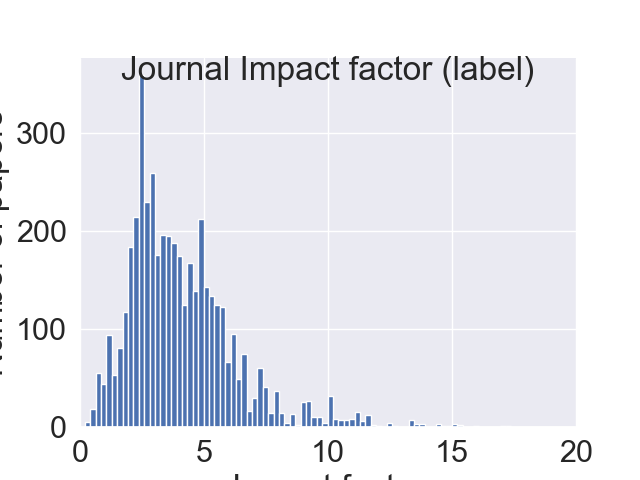
\includegraphics[width= \columnwidth]{./Images/JIF_hist.png}
	\caption{Overlaid distributions of observed and predicted values for the best model.}
	\label{fig:JIF_hist}
\end{figure}

Comparing distribution of the predicted JIFs and the observed values (Figure~\ref{fig:JIF_hist}) we can see that distribution of the predicted values is a lot closer to normal than the distribution of the observed. Two departures from the normality for the observed values are immediately obvious: spikes in the frequency at JIFs 1 and 2.5. Our model failed to capture these two features. Instead, those papers that should have been in those spikes were assigned higher JIF resulting in over-prediction for JIFs around 4.  Consequently, the correlation between predicted and observed values is far from perfect (Figure~\ref{fig:best_model_corr}). 

Cursory examination of the mispredicted records yield a plausible explanation. Some journals, in particular those with lower rank, allow for much longer abstracts, essentially turning the abstract into a mini-paper, including sections on experimental details, methods and discussion. This is not a standard practice, most other journals require abstract to be under 250 words and convey only general idea of the paper. The model likely assigned higher value to these unusually high quality abstracts. This hypothesis is partially confirmed by the modelling of the prediction error (\textit{vide infra}).

To elucidate the role of various factors in making erroneous predictions, we built a series of simple linear models predicting the difference between observed and predicted JIF. The only factor that had reasonable predictive power (r = 0.71 for observed and predicted error) was the journal name. Interestingly, very different kinds of journals had the same coefficient explaining the error: prestigious "Proceedings of the National Academy of Science" was under-predicted by the same factor as an obscure "Chinese Chemical Letters". Some of this can be explained by the phenomenon mentioned above, but some of the journals are prone to error because their impact factor is influenced by factors not included in the model. For instance, "Chinese Chemical Letters" publish a lot of reviews than naturally have much higher impact factor, thus pushing overall journal impact factor up. We explicitly excluded reviews from our analysis and could not capture this trend.

\begin{figure}
	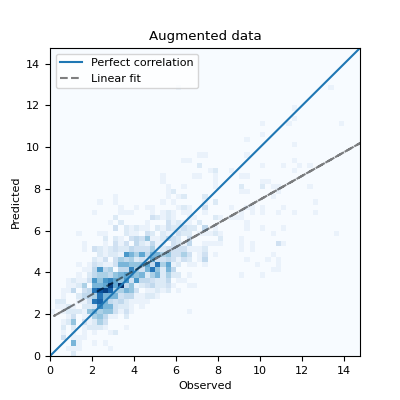
\includegraphics[width= \columnwidth]{./Images/Best model.png}
	\caption{Observed-Predicted correlation for the best model.}
	\label{fig:best_model_corr}
\end{figure}

\section{Conclusions and Next Steps}
Our preliminary experiments strongly support rejection of our somewhat cynical null hypothesis. More to that, performance of our best model approaches useful, with more than 70\% correlation between predicted and observed, this model can give the researcher a good estimate of what journals are good fit for their paper. 
To improve observed-predicted correlation we plan to investigate using sentence-level cls-tokens as well as full set of word embeddings, possibly in combination with CNN architecture. To combat over fitting we plan to enrich data set by adding concatenating titles to abstracts. As a long-shot experiment we also plan to augment data with synthetic abstracts compiled from individual sentences of papers published in the same journal in the same year.

Target variable transformation might be beneficial as well. Presently we use linear regression, which might produce negative values. By replacing JIF with JIF rank calculated on the training data set and using sigmoid activation on the output layer, we might achieve improved model performance. 

% Entries for the entire Anthology, followed by custom entries
\bibliography{custom}
\bibliographystyle{acl_natbib}

\end{document}
